% Chapter 5
\chapter{پیاده‌سازی و بررسی نتایج}

\section{مقدمه}
تست



\section{پیاده‌سازی مدل‌های شبکه عصبی}
در این بخش، دو ساختار و مدل اصلی شبکه‌های عصبی که طراحی شده‌اند، مورد بررسی قرار خواهند گرفت. این دو ساختار اصلی شامل شبکه عصبی پرسپترون چندلایه%
\LTRfootnote{Multilayer Perceptron}
\lr{(MLP)}
و شبکه عصبی پیچشی%
\LTRfootnote{Convolutional Neural Network}
\lr{(CNN)}
می‌باشند. در ادامه، هر یک از این مدل‌های طراحی شده به صورت مفصل توضیح داده خواهند شد. این توضیحات به منظور فراهم آوردن درکی جامع از نحوه عملکرد هر مدل و نقش آن‌ها در بررسی نتایج و مقایسه روش‌ها در پژوهش انجام خواهد شد. استفاده از این مدل‌ها به تحلیل و ارزیابی دقیق‌تر نتایج کمک کرده و مقایسه‌ای جامع از روش‌های مختلف را ممکن می‌سازد.

\subsection{
	مدل
	\lr{MLP}
}
در شبکه عصبی چندلایه تعریف شده، ابتدا لایه‌های شبکه عصبی در قالب یک ساختار ترتیبی%
\LTRfootnote{Sequential}
با استفاده از یک دیکشنری مرتب%
\LTRfootnote{OrderedDict}
تعریف می‌شوند. این ساختار ترتیب‌دار باعث می‌شود که لایه‌ها به صورت متوالی اجرا شوند و خروجی هر لایه به عنوان ورودی به لایه بعدی منتقل شود.

اولین لایه، یک لایه کاملاً متصل است که تعداد نورون‌های ورودی آن برابر با تعداد ویژگی‌های ورودی مدل به صورت تخت‌شده%
\LTRfootnote{Flatten}
و تعداد نورون‌های خروجی آن 256 است. این لایه تمام اتصالات ممکن بین نورون‌های ورودی و خروجی را دارد. پس از این لایه، یک تابع فعال‌سازی 
\lr{ReLU}
قرار دارد که وظیفه آن این است که تمامی مقادیر منفی خروجی را به صفر تبدیل کند و مقادیر مثبت را بدون تغییر نگه دارد.

لایه دوم، یک لایه کاملاً متصل دیگر است که 256 نورون ورودی و 128 نورون خروجی دارد. پس از این لایه نیز یک تابع فعال‌سازی
\lr{ReLU}
قرار دارد که مشابه تابع فعال‌ساز قبلی عمل می‌کند. سومین لایه نیز دقیقا مشابه لایه دوم است با این تفاوت که 128 نورون به عنوان ورودی و 64 نورون به عنوان خروجی دارد و در ادامه آن هم تابع فعال‌سازی
\lr{ReLU}
وجود دارد.

چهارمین و آخرین لایه، یک لایه کاملاً متصل است که 64 نورون ورودی و تعداد نورون‌های خروجی آن برابر با تعداد کلاس‌های موجود در مسئله طبقه‌بندی است. این لایه خروجی‌های نهایی شبکه را تولید می‌کند که نشان‌دهنده میزان تعلق هر ورودی به هر یک از کلاس‌ها است.

در نهایت، یک لایه 
\lr{Softmax}
اضافه شده است که وظیفه آن تبدیل خروجی‌های نهایی شبکه به توزیع احتمالاتی است. این لایه کمک می‌کند تا بتوان احتمال تعلق هر ورودی به هر کلاس را به صورت عددی بین صفر و یک بدست آورد که جمع کل این احتمالات برای همه کلاس‌ها برابر با یک خواهد بود. این توزیع احتمالاتی برای انجام پیش‌بینی‌های نهایی مورد استفاده قرار می‌گیرد. در پایان می‌توانید ساختار این مدل را در شکل
\ref{mlp}
مشاهده نمایید.

\begin{figure}[b!]
	\centering
	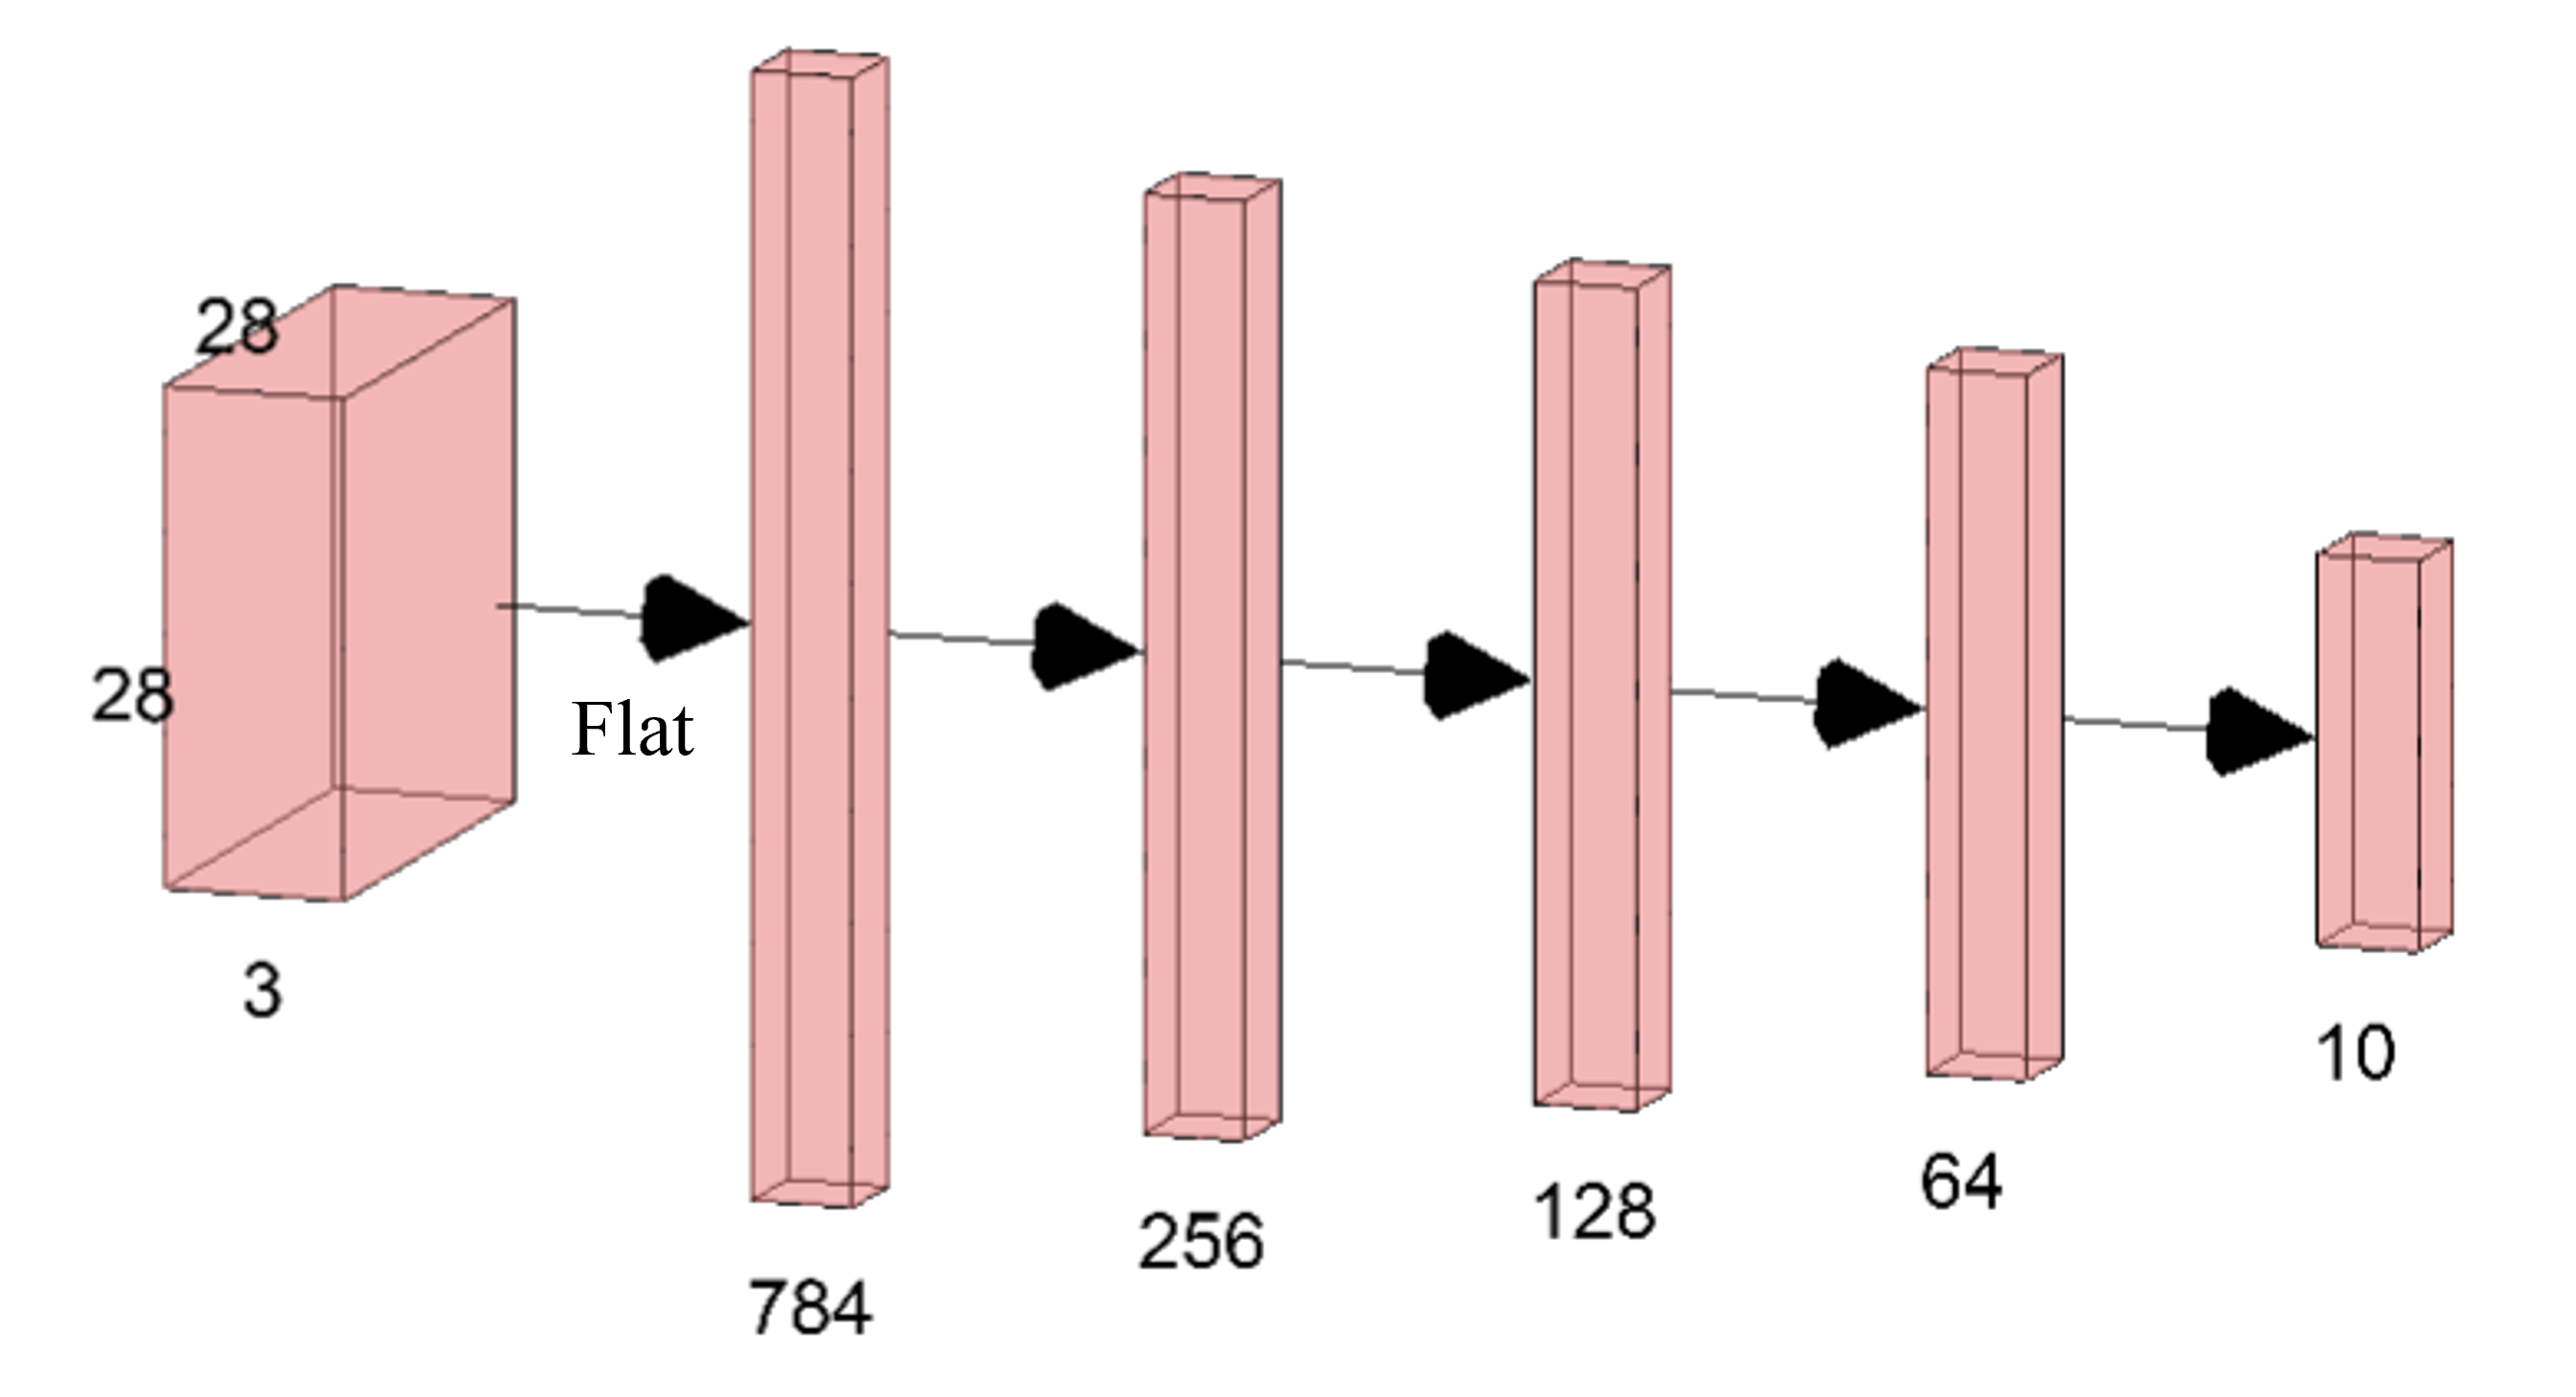
\includegraphics[scale=0.7]{images/chap5/mlp.png}%
	\caption{
		ساختار مدل 
		\lr{MLP}
	}
	\label{mlp}
	\centering
\end{figure}



\subsection{
	مدل
	\lr{CNN}
}
در شبکه عصبی پیچشی، ابتدا یک بلوک ترتیبی شامل لایه‌های مختلف به کمک دیکشنری مرتب تعریف شده است. این لایه‌ها به ترتیب وظایف مختلفی در استخراج ویژگی‌ها و انجام طبقه‌بندی نهایی دارند.

اولین لایه، یک لایه پیچشی تعریف شده است که تعداد کانال‌های ورودی تصویر را به 32 کانال خروجی تبدیل می‌کند. این لایه از یک کرنل ‎پیچشی با اندازه
3$\times$3
استفاده می‌کند. این لایه وظیفه دارد تا ویژگی‌های ابتدایی تصویر ورودی را استخراج کند. پس از این لایه، یک تابع فعال‌سازی 
\lr{ReLU}
قرار دارد که مقادیر منفی را به صفر تبدیل کرده و مقادیر مثبت را بدون تغییر نگه می‌دارد که این کار باعث ایجاد غیرخطی‌ شدن شبکه می‌شود.

سپس یک لایه تجمیع حداکثر%
\LTRfootnote{Max Pooling}
قرار دارد که اندازه فضای ویژگی‌های خروجی را کاهش می‌دهد و به کم کردن تعداد پارامترها و افزایش کارایی مدل کمک می‌کند. این لایه با انتخاب حداکثر مقدار در هر ناحیه کوچک
2$\times$2،
منجر به کاهش ابعاد تصاویر خواهد شد.

در ادامه، یک لایه پیچشی دیگر قرار دارد که تعداد کانال‌های خروجی را به 64 کانال افزایش می‌دهد. این لایه نیز از یک کرنل پیچشی با اندازه
3$\times$3
استفاده می‌کند و وظیفه استخراج ویژگی‌های پیچیده‌تر را بر عهده دارد. پس از این لایه نیز یک تابع فعال‌سازی
\lr{ReLU}
قرار دارد که مشابه قبل عمل می‌کند.

سپس یک لایه تجمیع حداکثر دیگر قرار دارد که اندازه فضای ویژگی‌های خروجی را مجدداً کاهش می‌دهد. این لایه نیز با انتخاب حداکثر مقدار در هر ناحیه کوچک
2$\times$2،
به کاهش ابعاد تصاویر کمک می‌کند.

پس از این لایه‌ها، یک لایه تخت‌کننده قرار دارد که ویژگی‌های چند بعدی خروجی را به یک بردار یک بعدی تبدیل می‌کند. این کار برای آماده‌سازی داده‌ها جهت ورود به لایه‌های کاملاً متصل انجام می‌شود.

در مرحله بعد، یک لایه کاملاً متصل قرار دارد که بردار ویژگی‌ها را به یک بردار با 100 نورون تبدیل می‌کند. این لایه تمام اتصالات ممکن بین نورون‌های ورودی و خروجی را دارد. پس از این لایه، یک تابع فعال‌سازی
\lr{ReLU}
وجود دارد که مشابه توابع فعال‌سازی قبلی عمل می‌کند و غیرخطی‌بودن را به شبکه اضافه می‌کند.

در پایان، یک لایه کاملاً متصل دیگر قرار دارد که بردار ویژگی‌ها را به یک بردار جدید با تعداد نورون‌هایی برابر با تعداد کلاس‌ها تبدیل می‌کند. این لایه، خروجی نهایی شبکه را تولید می‌کند که نشان می‌دهد هر ورودی به چه میزان به هر یک از کلاس‌ها تعلق دارد.

در انتها، یک لایه
\lr{Softmax} 
قرار داده شده که خروجی‌های نهایی شبکه را به توزیع احتمالاتی تبدیل می‌کند. این لایه باعث می‌شود که احتمال تعلق هر ورودی به هر کلاس به صورت عددی بین صفر و یک محاسبه شود، به طوری که مجموع این احتمالات برای همه کلاس‌ها برابر با یک باشد. این توزیع احتمالاتی در انتها برای انجام پیش‌بینی‌های نهایی به کار می‌رود. در پایان جهت درک بهتر می‌توانید ساختار این مدل را در شکل
\ref{cnn}
مشاهده نمایید.


\begin{figure}[t]
	\centering
	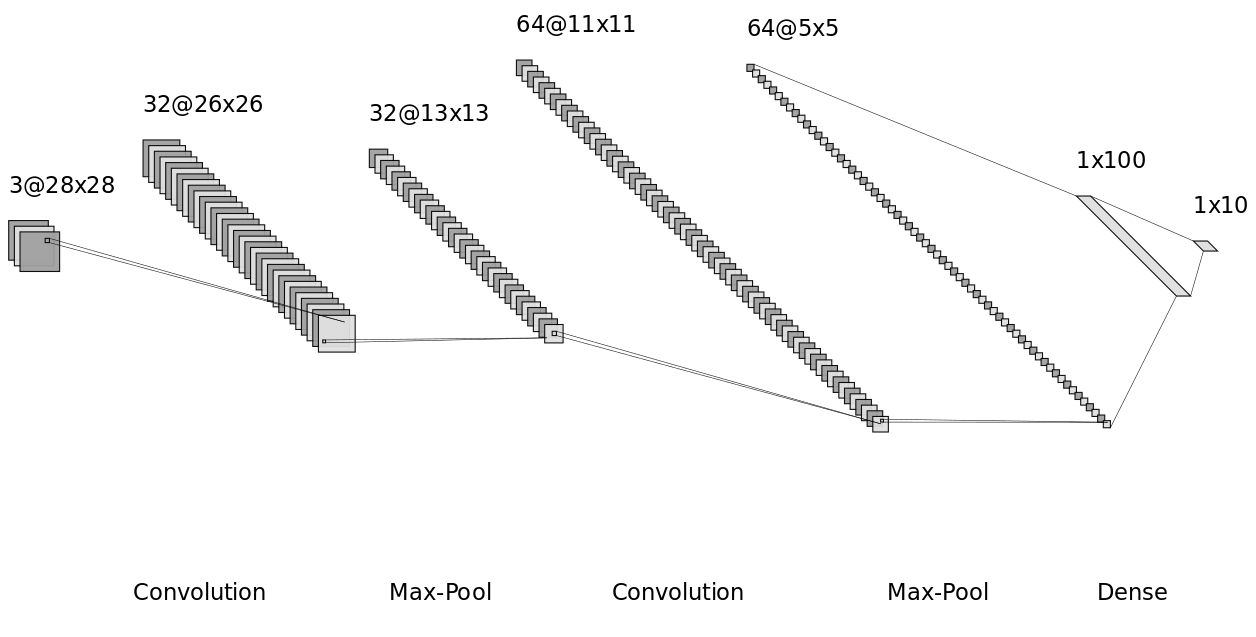
\includegraphics[scale=0.47]{images/chap5/cnn.png}%
	\caption{
		ساختار مدل 
		\lr{CNN}
	}
	\label{cnn}
	\centering
\end{figure}




\section{
	معرفی انواع مجموعه داده و مقایسه روش
	\lr{\texttt{\fontspec{Times New Roman} SimFedSwap}}
	با روش‌های پایه
}
در این پژوهش از انواع مجموعه داده‌ها برای بررسی و ارزیابی روش مورد نظر استفاده شده است. این مجموعه داده‌ها هر یک ویژگی‌های منحصر به فردی دارند که به تحلیل‌های دقیق‌تر و جامع‌تر کمک می‌کنند. در ادامه، هر یک از این مجموعه داده‌ها به طور مفصل معرفی و توضیح داده خواهد شد تا اهمیت و کاربردهای آن‌ها مشخص گردد.

تست ... کامل شود

تست ... کامل شود

\subsection{
مجموعه داده
	\lr{MNIST}%
	\LTRfootnote{Modified National Institute of Standards and Technology}
}
مجموعه داده
\lr{MNIST}
یکی از مشهورترین و پر استفاده‌ترین مجموعه داده‌ها در زمینه یادگیری ماشین است. این مجموعه شامل تصاویر دست‌نویس از اعداد 0 تا 9 می‌باشد و به طور گسترده‌ای برای آموزش و ارزیابی مدل‌های مختلف یادگیری ماشین به کار گرفته می‌شود.
مجموعه داده
\lr{MNIST}
در دهه 1990 توسط یان لکون%
\LTRfootnote{Yann LeCun}،
کورینا کورتس%
\LTRfootnote{Corinna Cortes}
و کریستوفر برجس%
\LTRfootnote{Christopher Burges}
 ایجاد شد. هدف اصلی این مجموعه داده، فراهم کردن یک مجموعه استاندارد برای ارزیابی الگوریتم‌های یادگیری ماشین و بینایی کامپیوتر بود.

مجموعه داده
\lr{MNIST}
شامل 70٬000 تصویر از ارقام دست‌نویس است که به دو بخش شامل مجموعه آموزش با 60٬000 تصویر و مجموعه تست با 10٬000 تصویر تقسیم می‌شود. هر تصویر دارای ابعاد
28$\times$28
پیکسل است که به صورت خاکستری%
\LTRfootnote{Grayscale}
ذخیره شده‌اند و هر پیکسل دارای مقداری بین 0 (سیاه) تا 255 (سفید) است. همچنین تمامی تصاویر با یک برچسب عددی بین 0 تا 9 همراه هستند که نمایانگر رقم موجود در تصویر می‌باشد
\cite{lecun1998gradient}.
چند نمونه از اعضای این مجموعه داده در شکل
\ref{mnist}%
، نمایش داده شده‌اند.

\begin{figure}[t]
	\centering
	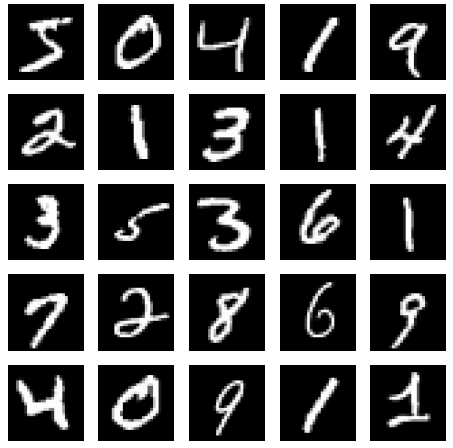
\includegraphics[scale=0.5]{images/chap5/mnist.png}%
	\caption{%
		چند نمونه از اعضای مجموعه داده
		\lr{MNIST}
		\cite{holzer2023dynamically}.
	}
	\label{mnist}
	\centering
\end{figure}


داده‌ها معمولاً در قالب دو فایل باینری شامل یکی برای تصاویر و دیگری برای برچسب‌ها ذخیره می‌شوند. هر تصویر به صورت یک بردار از اعداد بین 0 تا 255 با طول 784
(28$\times$28)
ذخیره می‌شود. به دلیل یکنواختی تصاویر و اندازه کوچک آن‌ها، نیاز به پیش‌پردازش پیچیده‌ای ندارند. یکی از مراحل پیش‌پردازش شامل نرمال‌سازی یا همان تبدیل مقادیر پیکسل‌ها به مقادیر بین 0 و 1 می‌باشد.

مجموعه داده
\lr{MNIST}
به عنوان یک نقطه شروع استاندارد برای آموزش و ارزیابی مدل‌های مختلف یادگیری عمیق و شبکه‌های عصبی استفاده می‌شود. محققان اغلب از
\lr{MNIST}
برای مقایسه کارایی الگوریتم‌های جدید با الگوریتم‌های موجود استفاده می‌کنند. این مجموعه شامل نمونه‌های متنوعی از ارقام دست‌نویس از افراد مختلف است که موجب می‌شود به عنوان یک معیار استاندارد برای مقایسه مدل‌ها و الگوریتم‌ها مورد استفاده قرار گیرد.

مجموعه داده
\lr{MNIST}
دارای مزایای زیادی از جمله سادگی، در دسترس بودن، استاندارد بودن و پراکندگی داده‌ها می‌باشد. با این حال، این مجموعه داده دارای معایبی نیز هست. به عنوان مثال، برای مسائل پیچیده‌تر و واقعی‌تر ممکن است
\lr{MNIST}
خیلی ساده باشد و نتواند چالش‌های واقعی را نشان دهد. همچنین، این مجموعه داده شامل تنها اعداد 0 تا 9 است و برای سایر کاربردهای دسته‌بندی تصویر ممکن است کافی نباشد.

کاربردهای عملی این مجموعه داده شامل آموزش شبکه‌های عصبی متفاوت برای بهبود دقت دسته‌بندی، تست و ارزیابی مدل‌های مختلف یادگیری عمیق و الگوریتم‌های بهینه‌سازی است. بسیاری از مدل‌ها و الگوریتم‌های پیشرفته امروزی با استفاده از مجموعه داده
\lr{MNIST}
توسعه و ارزیابی شده‌اند.

به طور کلی، مجموعه داده
\lr{MNIST}
با توجه به دلایل ذکر شده، یکی از مهم‌ترین و پراستفاده‌ترین مجموعه داده‌ها در زمینه یادگیری ماشین و بینایی کامپیوتر است. این مجموعه به محققان و دانشجویان کمک می‌کند تا مفاهیم پایه‌ای یادگیری ماشین را به خوبی درک کرده و الگوریتم‌های جدید را ارزیابی کنند.

در شکل 
\ref{result_mnist_mlp} 
نمونه‌ای از نتایج مقایسه روش 
\lr{SimFedSwap} 
با روش‌های پایه، بر روی مجموعه داده 
\lr{MNIST}
با استفاده از مدل
\lr{MLP}
نمایش داده شده است. همچنین پارامترهای استفاده شده در این اجرا نیز در جدول 
\ref{tabel_figMNIST} 
مشاهده می‌شوند. مورد مهمی که باید به آن توجه شود این است که منحنی‌های
\lr{FedAvg}
و
\lr{FedSwap}
به عنوان منحنی‌هایی نهایی و بر روی تمام دیگر منحنی‌ها رسم شده‌اند که در صورتی که رنگ دیگری در نمودار مشاهده شود،‌ به معنای بهتر یا بدتر بودن آن روش در آن نقطه از نمودار قابل بررسی و مقایسه باشد.

همان‌طور در شکل 
\ref{result_mnist_mlp}
مشاهده می‌شود، روش‌های مبتنی‌بر جابه‌جایی عملکرد بسیار اندکی بهتر از روش 
\lr{FedAvg} 
داشته‌اند. نکته مهم در این نتایج، عملکرد مشابه تمامی روش‌های مبتنی‌بر جابه‌جایی است. برای بررسی دقیق‌تر این اجرا، می‌توانید به منحنی‌های خطا در شکل 
\ref{app_result_mnist_mlp} 
پیوست مراجعه کنید.


\begin{figure}[h]
	\centering
	\subfigure[
	دید کلی از نتیجه
				\qquad\hspace{3mm}]{
		\label{result_mnist_mlp_mid}
		\includegraphics*[width=.48\textwidth]{images/chap5/result/mnist/acc_mid_1.png}
	}
	\hspace{0.8mm}
	\subfigure[
	بزرگ‌نمایی شده بخش اصلی					
				\qquad\hspace{5mm}]{
		\label{result_mnist_mlp_zoom}
		\includegraphics*[width=.48\textwidth]{images/chap5/result/mnist/acc_zoom_1.png}
	}
	\caption{
		مقایسه منحنی‌های دقت بر روی مجموعه داده
		\lr{MNIST}
		با استفاده از مدل
		\lr{MLP}.
	}
	\label{result_mnist_mlp}
\end{figure}


%\addtolength{\tabcolsep}{-0.5mm}
\begin{table}[h]
	\centering
	\caption{
	پارامترهای اجرا بر روی مجموعه داده
	\lr{MNIST}
	}
	\label{tabel_figMNIST}
%	\scalebox{0.985}{
	\begin{tabular}{ccccccccccccc}
		\hline
		\specialcell{مجموعه\\داده} &
		\specialcell{نحوه\\جابه‌جایی} &
		\specialcell{توزیع\\داده} &
		$K$ &
		$B$ &
		$C$ &
		$SP$ &
		$\eta$ &
		$E$ &
		$h_1$ &
		$h_2$
		\\
		\hline
		\lr{MNIST} &
		\lr{MSS} &
		نرمال &
		\lr{10} &
		\lr{32} &
		\lr{1.0} &
		\lr{1.0} &
		\lr{0.001} &
		\lr{1} &
		\lr{5} &
		\lr{3}
		\\
	\end{tabular}
%	}
\end{table}


%در ادامه در شکل
%\ref{result_mnist_mlp}
%دقیقا همان اجرای قبلی تکرار شده با این تفاوت که مدل شبکه عصبی به
%\lr{CNN}
%تغییر پیدا کرده است. همان‌طور که مشاهده می‌شود در این جا تقریبا تمامی روش‌ها مشابه هم عمل کرده‌اند. که می‌توان به این نکته اشاره کرد که در صورتی که شبکه به راحتی به درصد بالایی در دقت رسیده باشد، همگی روش‌ها مشابه یکدیگر خواهند بود. برای بررسی دقیق‌تر این اجرا، می‌توانید به منحنی‌های خطا در شکل 
%\ref{app_result_mnist_mlp} 
%پیوست مراجعه کنید.


\subsection{
	مجموعه داده
	\lr{CIFAR-10}%
	\LTRfootnote{Canadian Institute For Advanced Research}
}
مجموعه داده
\lr{CIFAR-10}
یکی از معروف‌ترین و پرکاربردترین مجموعه داده‌های مورد استفاده در حوزه یادگیری ماشین و بینایی کامپیوتر است. این مجموعه داده توسط گروهی به سرپرستی الکس کریژفسکی%
\LTRfootnote{Alex Krizhevsky}
و جفری هینتون%
\LTRfootnote{Geoffrey Hinton}
در دانشگاه تورنتو گردآوری شده و برای ارزیابی و آزمایش مدل‌های یادگیری عمیق به کار می‌رود.


مجموعه داده
\lr{CIFAR-10}
شامل 60٬000 تصویر رنگی با اندازه
32$\times$32
پیکسل است که به 10 کلاس مختلف تقسیم شده‌اند. هر کلاس شامل 6٬000 تصویر است که به صورت مساوی بین مجموعه‌های آموزشی و آزمایشی توزیع شده‌اند. این کلاس‌ها شامل مواردی مانند هواپیما، اتومبیل، پرنده، گربه، گوزن، سگ، قورباغه، اسب، کِشتی و کامیون هستند. هر یک از این کلاس‌ها دارای تصاویری است که تنوع بالایی از زوایا، پس‌زمینه‌ها و شرایط نوری مختلف را شامل می‌شود
\cite{krizhevsky2009learning}.
در شکل
\ref{cifar10}%
، چند نمونه از هر کلاس در مجموعه داده
\mbox{\lr{CIFAR-10}}
به نمایش در آمده است.


\begin{figure}[t]
	\centering
	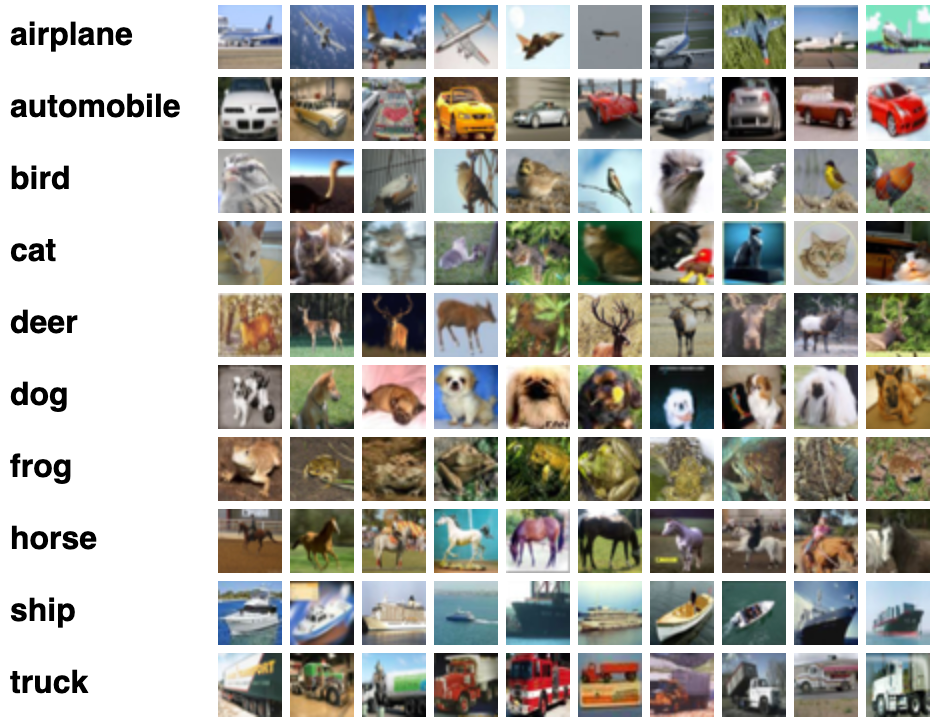
\includegraphics[scale=0.7]{images/chap5/cifar10.png}%
	\caption{%
		چند نمونه از هر کلاس در مجموعه داده
		\lr{CIFAR-10}
		\cite{Evan2022CIFAR10}.
	}
	\label{cifar10}
	\centering
\end{figure}



یکی از ویژگی‌های مهم مجموعه داده
\lr{CIFAR-10}
تنوع بالای تصاویر در هر کلاس است. این تنوع باعث می‌شود که مدل‌های یادگیری عمیق نیاز به توانایی تعمیم‌دهی بالا برای تشخیص صحیح کلاس‌ها داشته باشند. این مجموعه داده برای آموزش و ارزیابی مدل‌های مختلفی مورد استفاده قرار می‌گیرد و بسیاری از پژوهش‌ها و مقالات علمی از آن به عنوان مبنای مقایسه عملکرد مدل‌ها استفاده کرده‌اند.

مجموعه داده
\lr{CIFAR-10}
به دو بخش آموزشی و آزمایشی تقسیم شده است. بخش آموزشی شامل 50٬000 تصویر و بخش آزمایشی شامل 10٬000 تصویر است. این تقسیم‌بندی، استانداردی برای ارزیابی مدل‌ها فراهم می‌کند، به طوری که مدل‌ها می‌توانند بر روی مجموعه آموزشی، آموزش دیده و سپس بر روی مجموعه آزمایشی ارزیابی شوند. این روش به محققان امکان می‌دهد تا عملکرد مدل‌ها را به صورت عینی و قابل تکرار مقایسه کنند.

به دلیل اندازه کوچک تصاویر (%
32$\times$32
پیکسل)، پردازش و آموزش مدل‌ها بر روی
\lr{CIFAR-10}
نسبتاً سریع و کم هزینه است. این ویژگی باعث شده تا مجموعه داده 
\lr{CIFAR-10}
برای آزمایش مدل‌ها بسیار مناسب باشد. بسیاری از ابزارها و چارچوب‌های%
\LTRfootnote{Frameworks}
یادگیری ماشین مانند
\lr{PyTorch}
و
\lr{TensorFlow}
شامل توابع و ابزارهای آماده برای بارگذاری و استفاده از این مجموعه داده هستند که این امر نیز به سهولت استفاده از آن کمک می‌کند.

در نهایت، مجموعه داده
\lr{CIFAR-10}
با ارائه تصاویری متنوع و چالش‌برانگیز در کلاس‌های مختلف، ابزاری قدرتمند برای آموزش و ارزیابی مدل‌های یادگیری عمیق فراهم می‌کند. این مجموعه داده نه تنها در پژوهش‌های دانشگاهی بلکه در صنعت نیز به عنوان معیاری برای ارزیابی پیشرفت‌ها در حوزه بینایی کامپیوتر استفاده می‌شود.


\subsection{
	مجموعه داده
	\lr{CINIC-10}%
	\LTRfootnote{CIFAR-10 and ImageNet Combined}
}
مجموعه داده
\lr{CINIC-10}
یک مجموعه داده تصویری گسترده و متنوع است که برای ارزیابی عملکرد مدل‌های یادگیری ماشین به ویژه در زمینه‌های مرتبط با طبقه‌بندی تصاویر مورد استفاده قرار می‌گیرد. این مجموعه داده ترکیبی از تصاویر موجود در مجموعه‌ داده‌های معروف
\lr{CIFAR-10}
و
\lr{ImageNet}
است. این ترکیب به منظور ایجاد مجموعه‌ای گسترده‌تر و متنوع‌تر از تصاویر انجام شده است که می‌تواند به ارزیابی دقیق‌تر و واقع‌گرایانه‌تر مدل‌ها کمک کند.

مجموعه داده
\lr{CINIC-10}
شامل 270٬000 تصویر است که در 10 کلاس مختلف دسته‌بندی شده‌اند. هر کلاس شامل 27٬000 تصویر است که به دو بخش آموزشی و آزمایشی تقسیم شده‌اند. بخش آموزشی شامل 180٬000 تصویر و بخش آزمایشی شامل 90٬000 تصویر است. این تقسیم‌بندی منظم به محققان و مهندسان یادگیری ماشین این امکان را می‌دهد که به راحتی مدل‌های خود را آموزش داده، اعتبارسنجی و آزمایش کنند.

تصاویر موجود در
\lr{CINIC-10}
دارای ابعاد
32$\times$32
پیکسل هستند که مشابه ابعاد تصاویر موجود در مجموعه داده
\lr{CIFAR-10}
است. این ویژگی باعث می‌شود که مدل‌های از پیش آموزش دیده بر روی
\lr{CIFAR-10}
بتوانند به راحتی بر روی این مجموعه داده نیز مورد استفاده قرار گیرند و ارزیابی شوند. با این حال، تنوع بیشتر تصاویر در
\lr{CINIC-10}
نسبت به
\lr{CIFAR-10}
به دلیل ترکیب تصاویر از
\lr{ImageNet}،
چالشی جدی‌تر برای مدل‌های یادگیری ماشین فراهم می‌کند
\cite{darlow2018cinic}.
در شکل
\ref{cinic10}%
، تعدادی نمونه از کلاس خودرو در مجموعه داده
\mbox{\lr{CIFAR-10}}
به نمایش در آمده است.


\begin{figure}[b!]
	\centering
	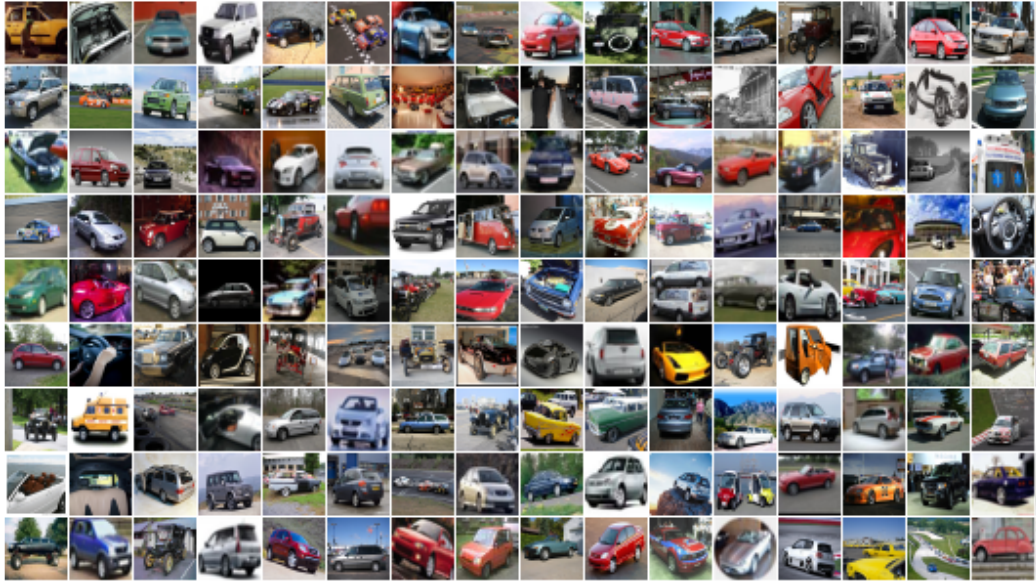
\includegraphics[scale=0.5]{images/chap5/cinic10.png}%
	\caption{%
		تعدادی نمونه از کلاس خودرو در مجموعه داده
		\lr{CINIC-10}
		\cite{darlow2018cinic}.
	}
	\label{cinic10}
	\centering
\end{figure}



یکی از اهداف اصلی ایجاد
\lr{CINIC-10}،
افزایش تنوع و پیچیدگی تصاویر مورد استفاده برای آموزش و ارزیابی مدل‌ها بود. این مجموعه داده شامل تصاویری از دنیای واقعی است که در شرایط نوری مختلف و با پس‌زمینه‌های متنوع گرفته شده‌اند. این ویژگی به مدل‌ها کمک می‌کند تا به جای این که تنها بر روی مجموعه‌ای محدود از تصاویر آموزش ببینند، توانایی تعمیم‌دهی خود را به تصاویر جدید و غیرمنتظره نیز افزایش دهند.

در نهایت،
\lr{CINIC-10}
با هدف ارتقای استانداردهای ارزیابی مدل‌های یادگیری عمیق و بهبود عملکرد آن‌ها در مواجهه با داده‌های واقعی و متنوع ایجاد شده است. این مجموعه داده به محققان این امکان را می‌دهد که مدل‌های خود را در شرایط نزدیک به دنیای واقعی آزمایش کرده و نقاط ضعف و قوت آن‌ها را بهتر شناسایی کنند. به همین دلیل،
\lr{CINIC-10}
به عنوان یک ابزار ارزشمند در جامعه یادگیری ماشین شناخته می‌شود و به طور گسترده‌ای مورد استفاده قرار می‌گیرد.


\subsection{
	مجموعه داده
	\lr{FEMNIST}%
	\LTRfootnote{Federated Extended MNIST}
}
مجموعه داده
\lr{FEMNIST}
یک مجموعه داده توسعه‌یافته از مجموعه مشهور
\lr{MNIST}
است که برای کاربردهای یادگیری فدرال طراحی شده است.
این مجموعه داده شامل 814٬255 تصویر است که در 62 کلاس مختلف دسته‌بندی شده‌اند و 10 درصد این داده‌ها به بخش آموزشی تعلق دارند. مجموعه داده
\lr{FEMNIST}
از تصاویر دست‌نوشته به وجود آمده است که شامل اعداد و حروف الفبای انگلیسی می‌شود.

برخلاف مجموعه داده
\lr{MNIST}
که تنها شامل اعداد دست‌نوشته از صفر تا نه است، مجموعه داده
\lr{FEMNIST}
شامل حروف بزرگ و کوچک الفبای انگلیسی نیز می‌باشد. این ویژگی باعث می‌شود که
\lr{FEMNIST}
نسبت به
\lr{MNIST}
تنوع بیشتری داشته باشد و برای آزمایش مدل‌های پیچیده‌، مناسب‌تر باشد
\cite{caldas2018leaf}.
چند نمونه از اعضای این مجموعه داده در شکل
\ref{femnist}%
، نمایش داده شده‌اند.
در این مجموعه داده، تعداد داده‌ها در هر کلاس یکسان نیست و کلاس‌های مختلف دارای تعداد متفاوتی از داده‌ها هستند. شکل
\ref{count_all_classes}%
، تعداد داده‌های هر کلاس و نحوه نام‌گذاری آن‌ها را نشان می‌دهد.


\begin{figure}[b!]
	\centering
	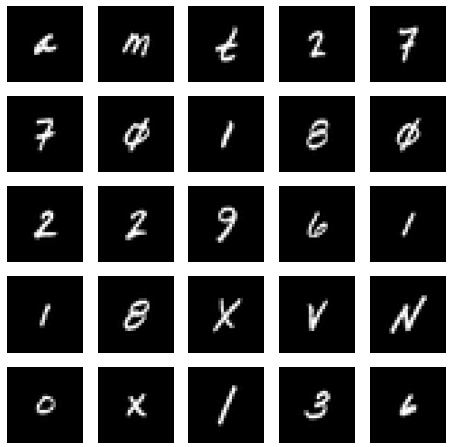
\includegraphics[scale=0.5]{images/chap5/femnist.png}%
	\caption{%
		چند نمونه از اعضای مجموعه داده
		\lr{FEMNIST}
		\cite{holzer2023dynamically}.
	}
	\label{femnist}
	\centering
\end{figure}


\begin{figure}[t]
	\centering
	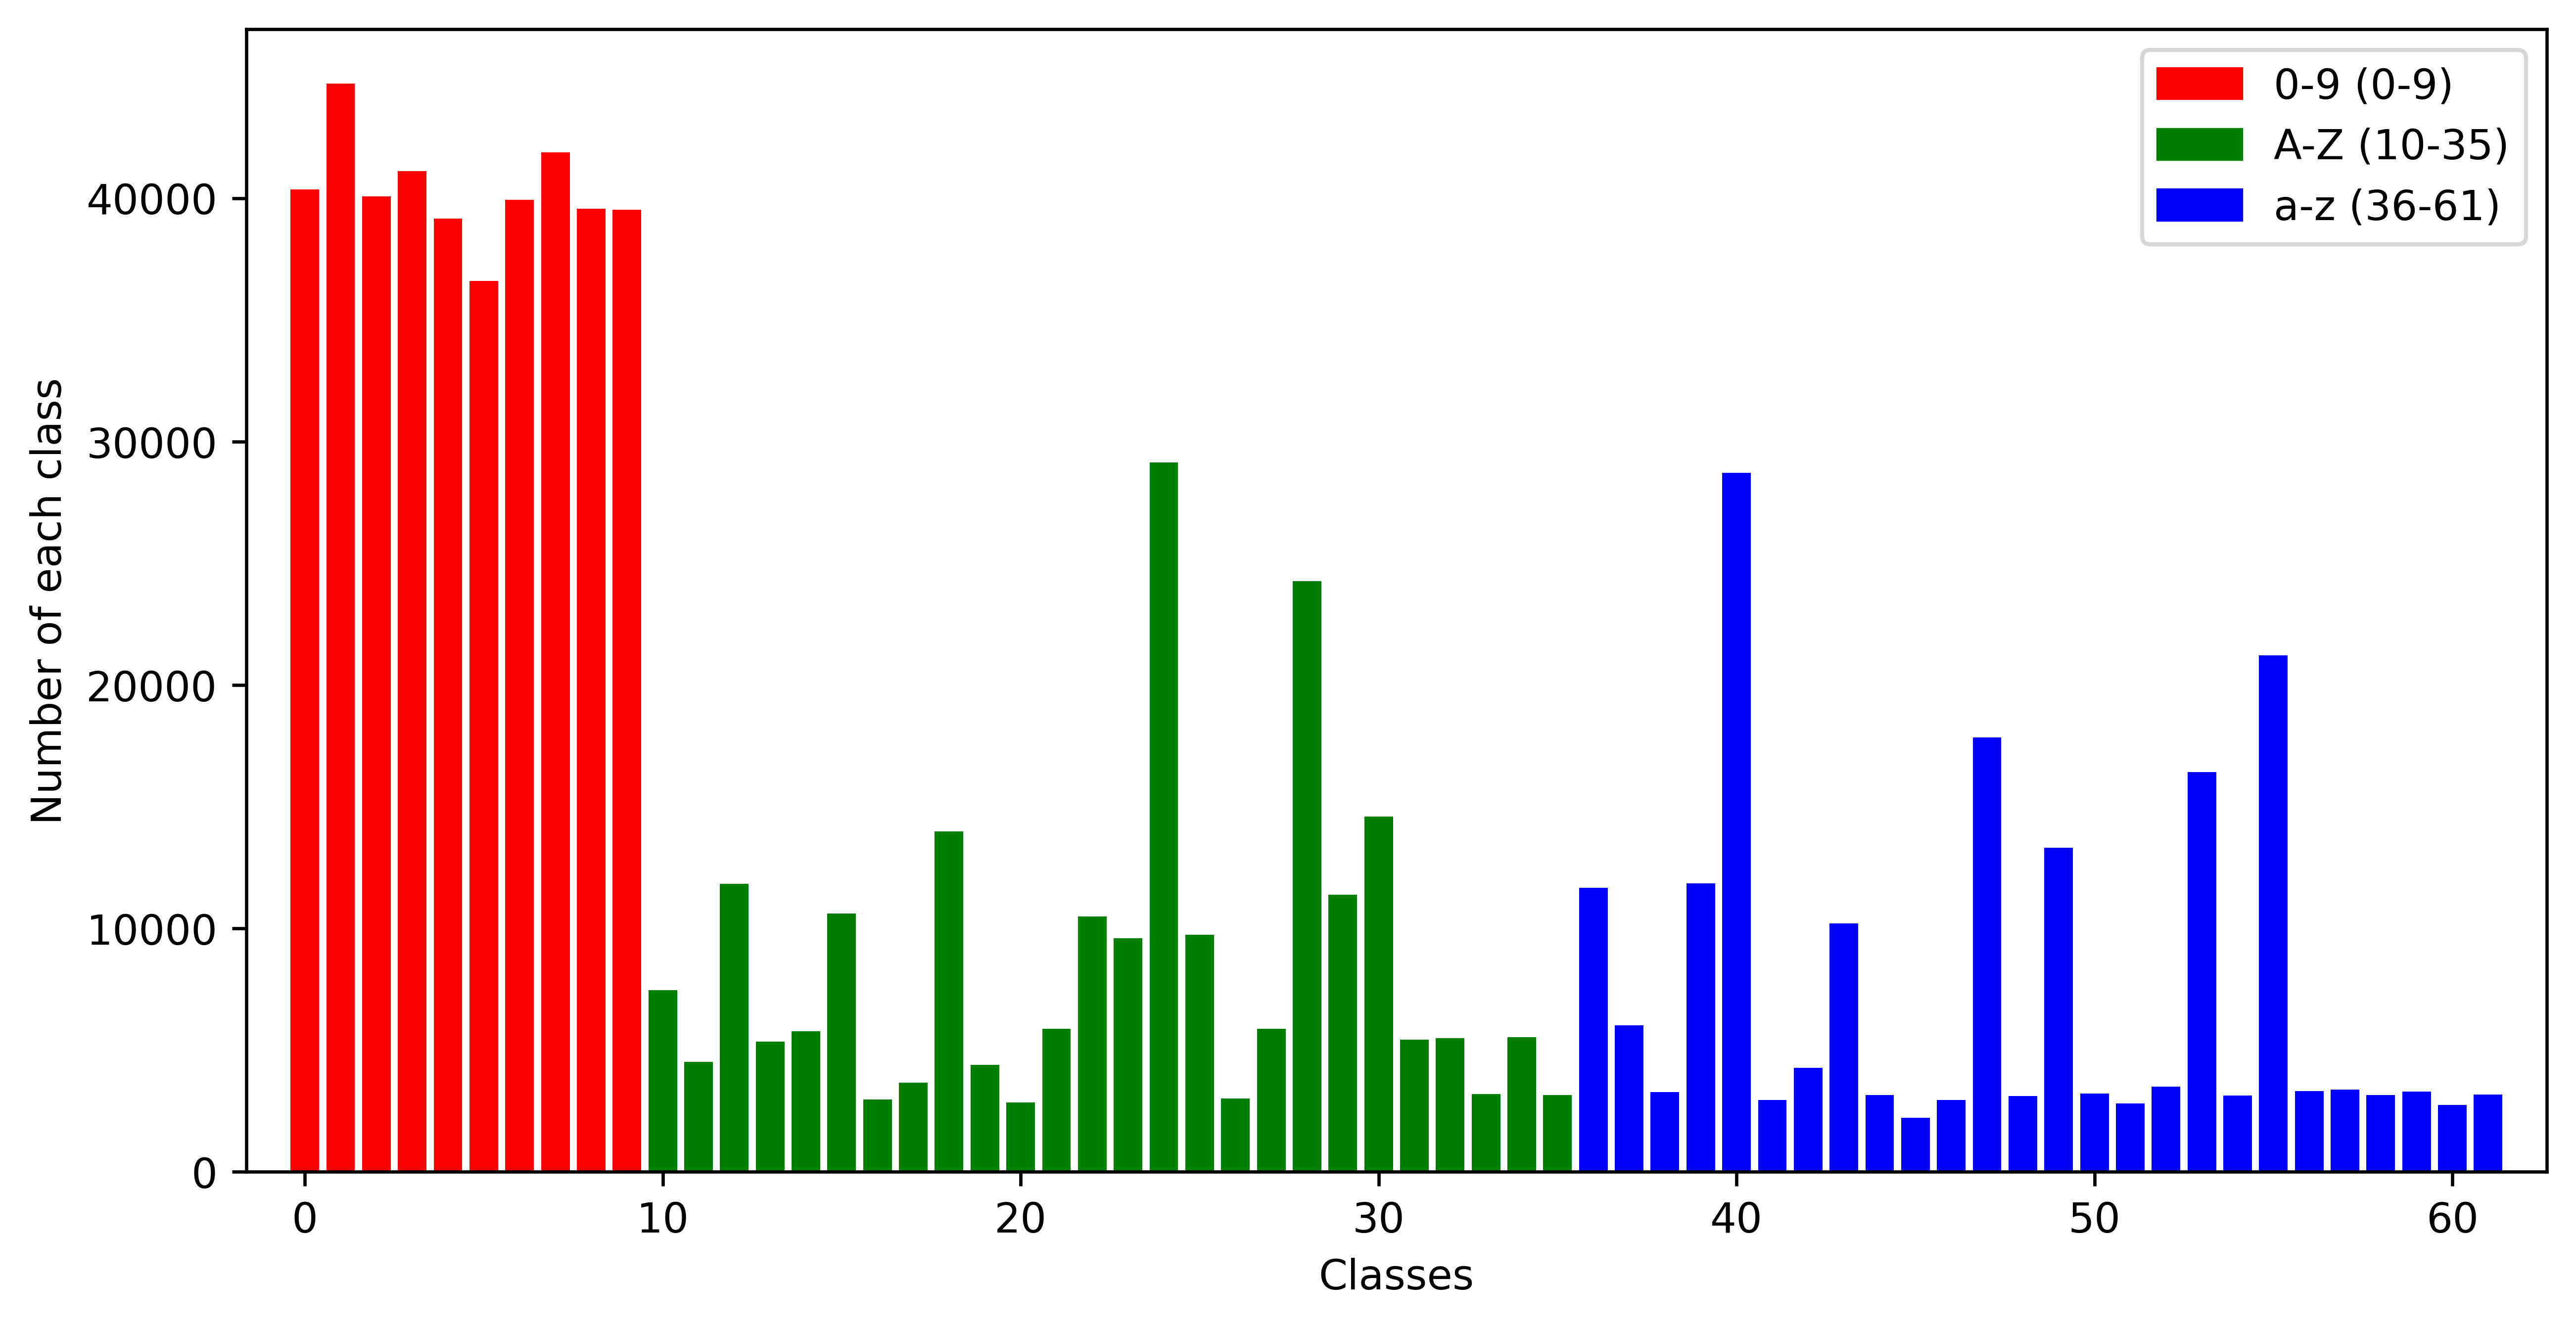
\includegraphics[scale=0.7]{images/chap5/count_all_classes.png}%
	\caption{%
تعداد داده‌های هر کلاس و نحوه نام‌گذاری در مجموعه داده
		\lr{FEMNIST}.
	}
	\label{count_all_classes}
	\centering
\end{figure}

همانطور که در شکل
\ref{count_all_classes}
مشاهده می‌شود، تعداد کلاس‌های 0 تا 9 که به ارقام 0 تا 9 اشاره دارند، به‌طور قابل‌توجهی بیشتر از سایر کلاس‌هاست و هر کدام حدود 40٬000 نمونه دارند. در بین کلاس‌های 10 تا 35 که مربوط به حروف بزرگ انگلیسی هستند، کلاس‌های \lr{S} و \lr{O} بیشترین تعداد نمونه را دارند. به نظر می‌رسد این سبک از جمع‌آوری داده به دلیل جلوگیری از اشتباه گرفتن کلاس \lr{O} با عدد صفر و کلاس \lr{S} با معادل حرف کوچک آن در کلاس‌های 36 تا 61 بوده باشد.


یکی از ویژگی‌های برجسته مجموعه داده
\lr{FEMNIST}،
نحوه سازماندهی داده‌ها است. این مجموعه داده بر اساس کاربران مختلف تقسیم‌بندی شده است، به طوری که هر کاربر دارای مجموعه‌ای از داده‌های دست‌نوشته خود است. این سازماندهی امکان آزمایش و ارزیابی روش‌های یادگیری فدرال را فراهم می‌کند، زیرا در یادگیری فدرال داده‌ها به صورت محلی بر روی دستگاه‌های کاربران، نگه‌داری می‌شوند و مدل‌ها بر روی این داده‌ها آموزش می‌بینند. این ویژگی به محققان اجازه می‌دهد تا سناریوهای واقعی‌تری از یادگیری فدرال را شبیه‌سازی و بررسی کنند.

مجموعه داده
\lr{FEMNIST}
به صورت پیش‌فرض شامل 3597 کاربر است که داده‌ها میان این کاربران توزیع شده‌اند. این توزیع نه از لحاظ تعداد تصاویر بین کاربران و نه از لحاظ پوشش‌دهی کلاس‌ها در هر کاربر، یکسان نیست. با این حال، تعداد کاربران و نحوه توزیع داده‌ها میان آنها را می‌توان به دلخواه تغییر داد.

برای بررسی حالت پیش‌فرض، می‌توان مشاهده کرد که هر کاربر چه تعداد کلاس را پوشش داده است. در شکل
\ref{clients_cover_classes}
قابل مشاهده است که هر کاربر چند کلاس را شامل می‌شود. به عنوان مثال، این شکل نشان می‌دهد که حدود 400 کاربر وجود دارند که هر کدام 58 کلاس را پوشش داده‌اند. همچنین برای بررسی تعداد تصاویری که در هر کاربر وجود دارد، می‌توان به شکل
\ref{clients_images}
توجه کرد. این شکل نشان می‌دهد که حدودا 480 کاربر وجود دارند که هر کدام 175 تصویر را شامل می‌شوند.



\begin{figure}[t]
	\centering
	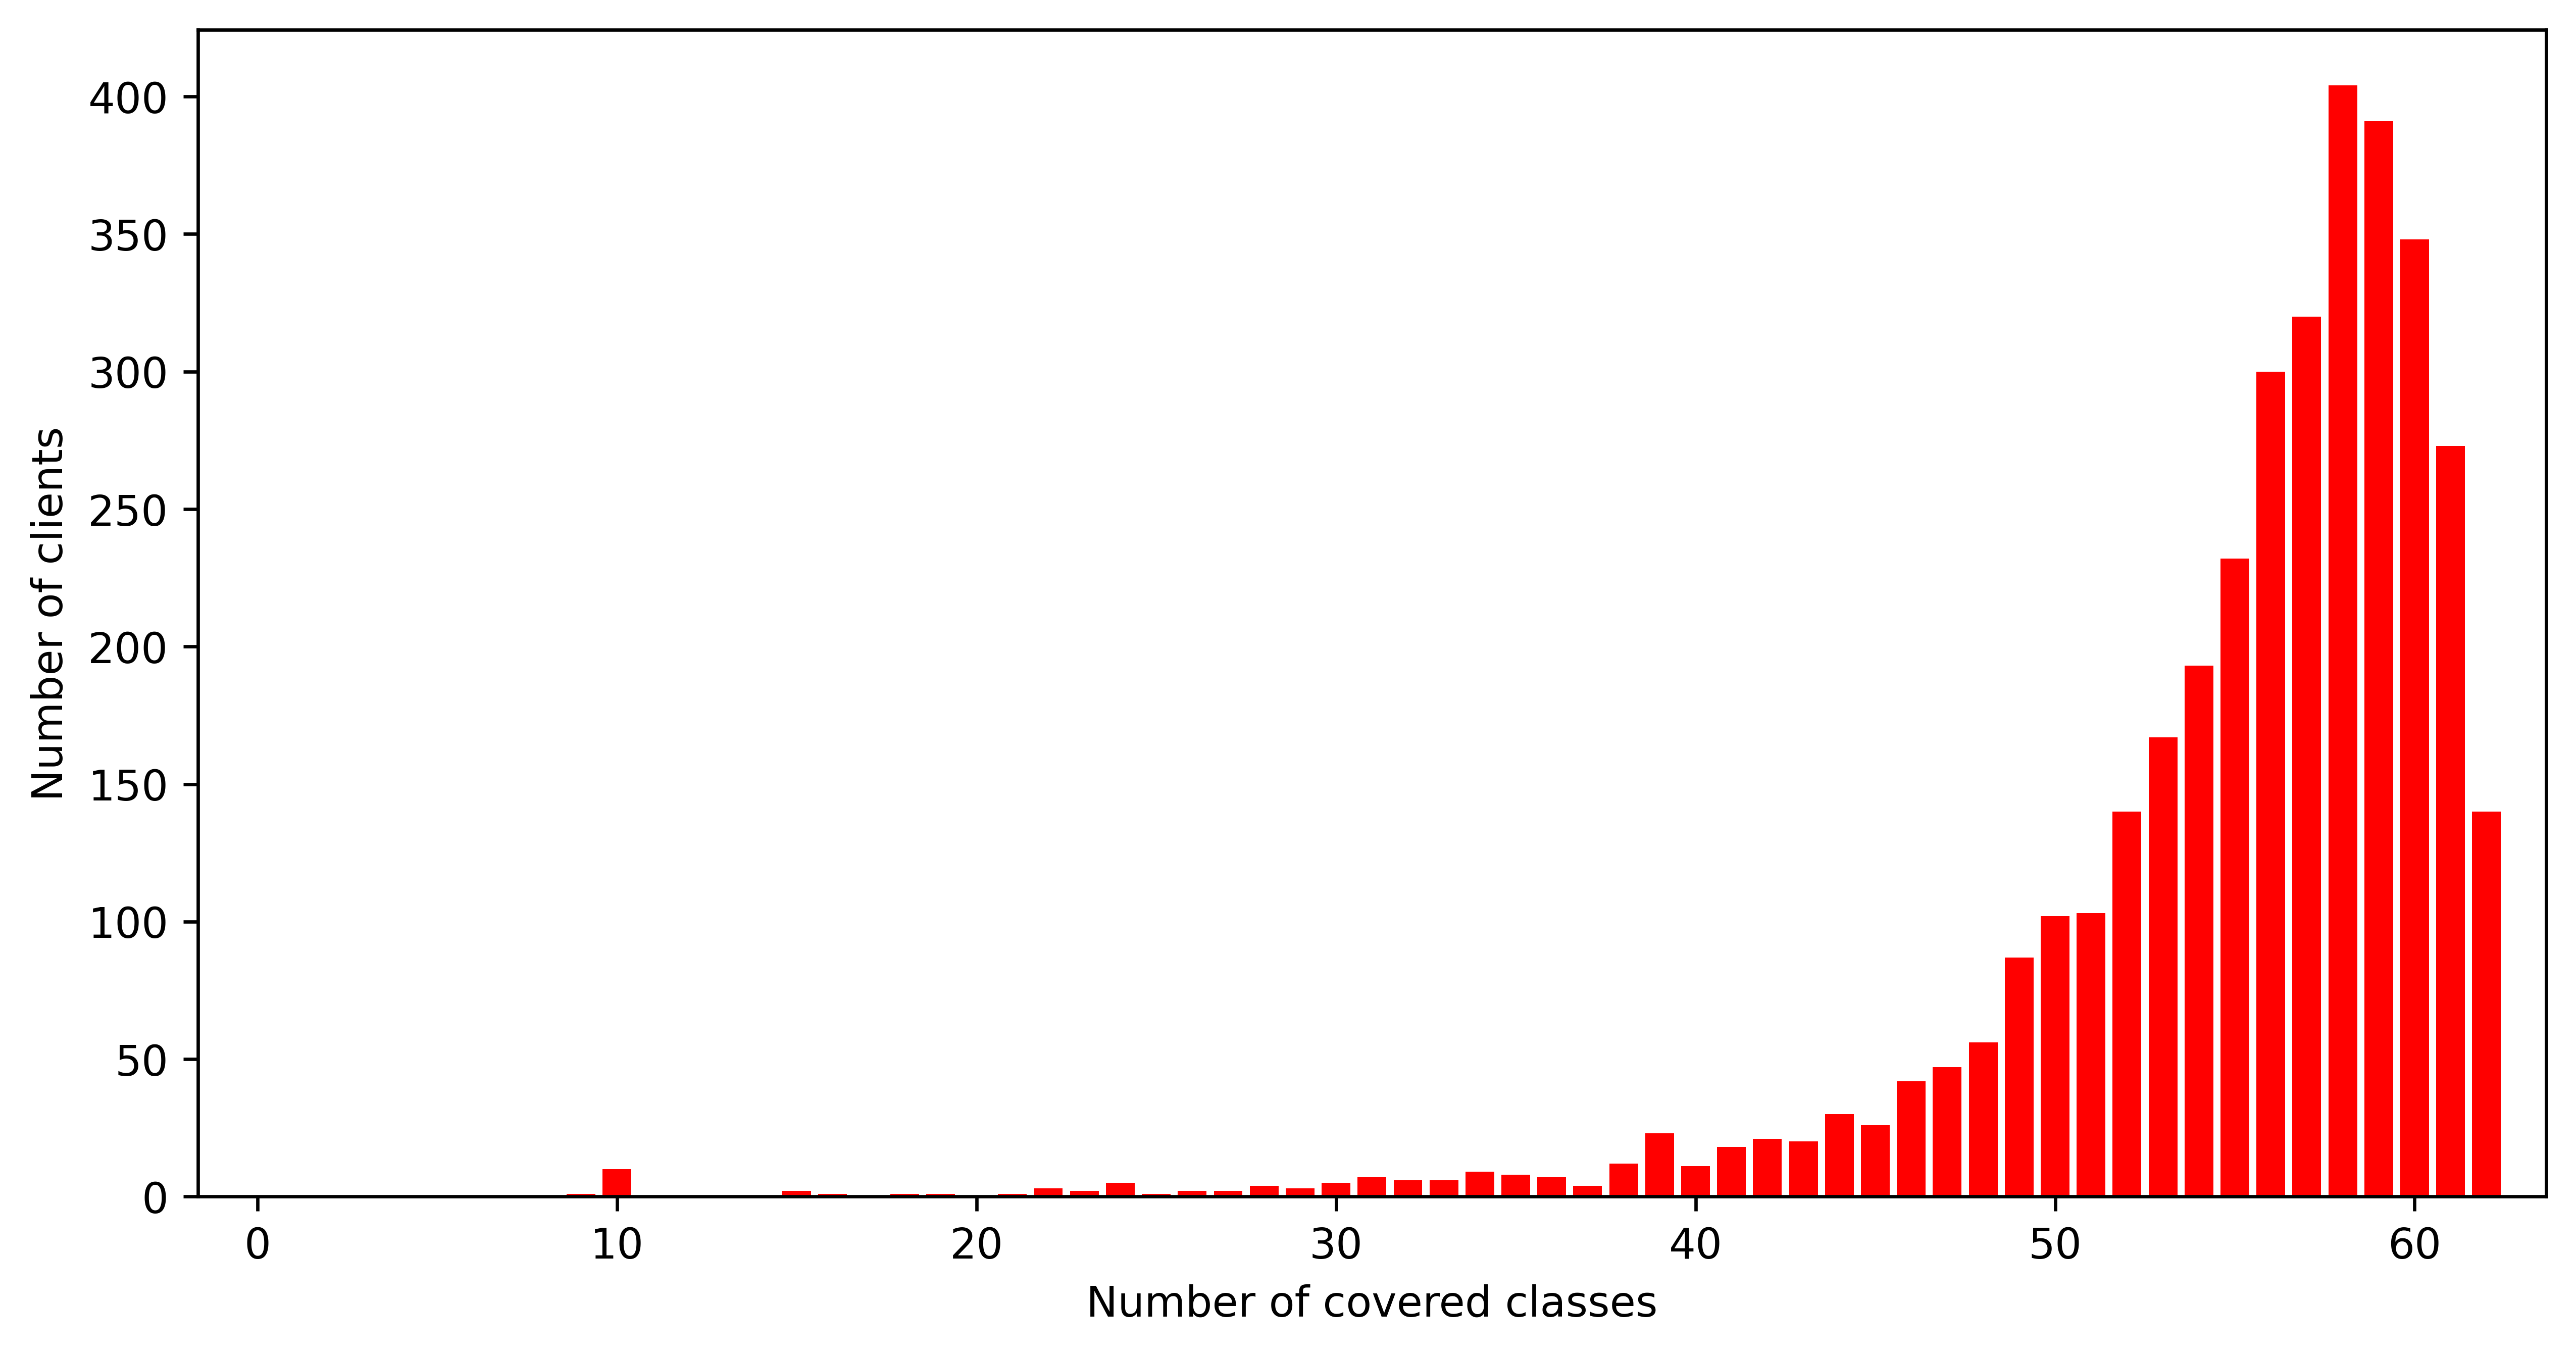
\includegraphics[scale=0.7]{images/chap5/clients_cover_classes.png}%
	\caption{%
تعداد کلاس‌های پوشش‌داده شده توسط کاربران در مجموعه داده
		\lr{FEMNIST}.
	}
	\label{clients_cover_classes}
	\centering
\end{figure}


\begin{figure}[t!]
	\centering
	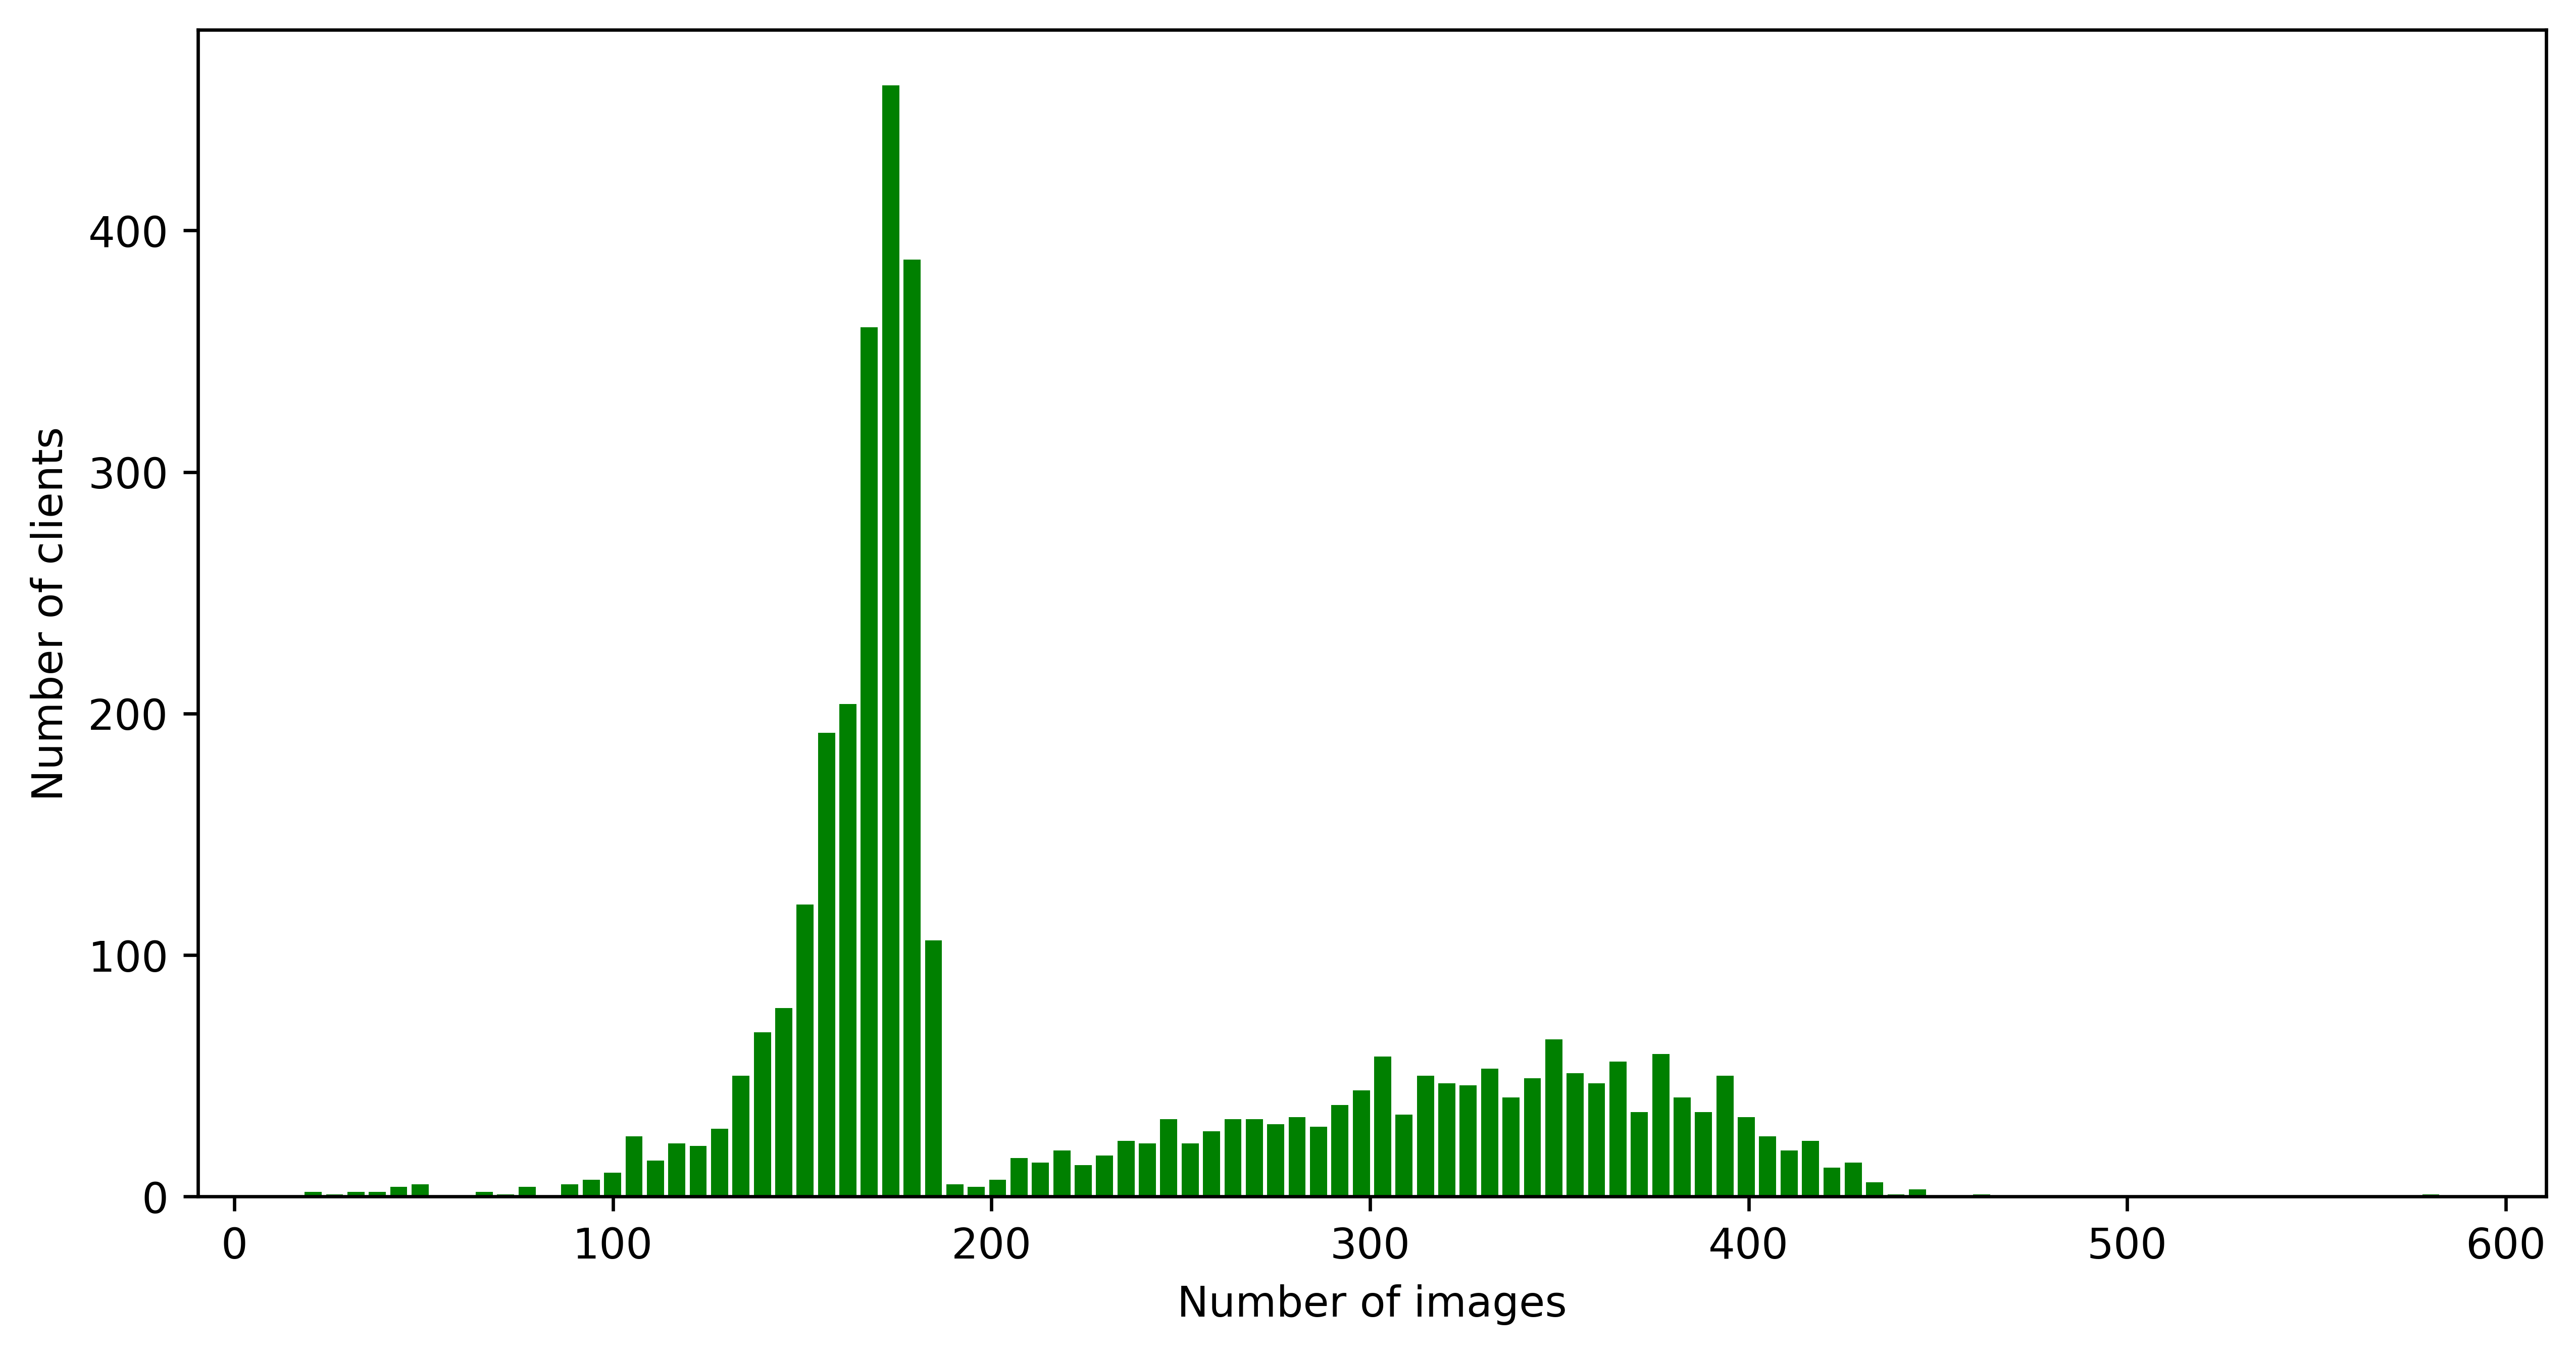
\includegraphics[scale=0.7]{images/chap5/clients_images.png}%
	\caption{%
		تعداد تصاویر هر یک از کاربران در مجموعه داده
		\lr{FEMNIST}.
	}
	\label{clients_images}
	\centering
\end{figure}



تصاویر در مجموعه داده
\lr{FEMNIST}
به صورت سیاه و سفید و با اندازه
28$\times$28
پیکسل هستند. هر تصویر نمایانگر یک کاراکتر دست‌نوشته است. این تصاویر از مجموعه داده
\lr{NIST}
استخراج شده‌اند و به صورت مناسبی برای کاربردهای یادگیری فدرال سازماندهی شده‌اند. در حقیقت این تصاویر شامل نویسه‌های مختلف از کاربران مختلف است که تنوع در سبک نوشتن و کیفیت دست‌نوشته‌ها را افزایش می‌دهد.


به طور کلی، مجموعه داده
\lr{FEMNIST}
یک ابزار قدرتمند برای تحقیقات در زمینه یادگیری فدرال است. با ارائه تنوع بالای داده‌ها و سازماندهی مناسب برای سناریوهای یادگیری فدرال، این مجموعه داده به محققان کمک می‌کند تا روش‌ها و الگوریتم‌های جدید را در محیط‌های واقعی‌تر آزمایش کنند. این ویژگی‌ها باعث شده تا
\lr{FEMNIST}
به عنوان یکی از مجموعه داده‌های مرجع در این حوزه شناخته شود و در بسیاری از تحقیقات علمی و صنعتی مورد استفاده قرار گیرد.




\section{
	مقایسه جابه‌جایی حریصانه با جابه‌جایی حداقل شباهت در روش
	\lr{\texttt{\fontspec{Times New Roman} SimFedSwap}}
}
تست
با توجه به شکل
\ref{mylabel1}
پیوست




\section{
	تحلیل کاهش تعداد کاربران در هر دور و افزایش تعداد کل دورها در روش
	\lr{\texttt{\fontspec{Times New Roman} SimFedSwap}}
}
تست


\section{جمع‌بندی}
اگر تعداد کاربران زیاد باشد، روش SimFedSwap می‌تواند کارایی خود را به نمایش بگذارد.








%
%با توجه به نتیجه
%\ref{mylabel1}
%
%
%\begin{figure}[t]
%	\centering
%	\subfigure[کل شکل\qquad\hspace{3mm}]{
%		\label{mylabel1}
%		\includegraphics*[width=.47\textwidth]{images/chap5/cinic10_r05_acc1.png}
%	}
%	\hspace{1.5mm}
%	\subfigure[بزرگ شده بخش انتهایی\qquad\hspace{5mm}]{
%		\label{mylabel2}
%		\includegraphics*[width=.47\textwidth]{images/chap5/cinic10_r05_acc2.png}
%	}
%	\caption{
%		تست
%		\lr{CINIC-10}
%	}
%	\label{mylabel}
%\end{figure}


